\section{Data processing and basic results}
\label{section:results}


In what follows, however, we will describe the performance 
of only read and write raw sensor data operations. The rest 
of the functionality is out of the scope.

We start with the data ingestion. Here, using the data source,
we were generating data points for random 1-hour period, and we were 
writing this data in batches. We have used Python threads
to simultaneously write data for 1, 10, and 50 tags (sensors)
at the same time. We computed the average number of 
samples per second and computed $95\%$ confidence intervals.

The results for write performance together with the $95\%$ confidence 
interval are shown in Figure~\ref{fig:write}. 

\begin{figure}[!hbt]\centering
  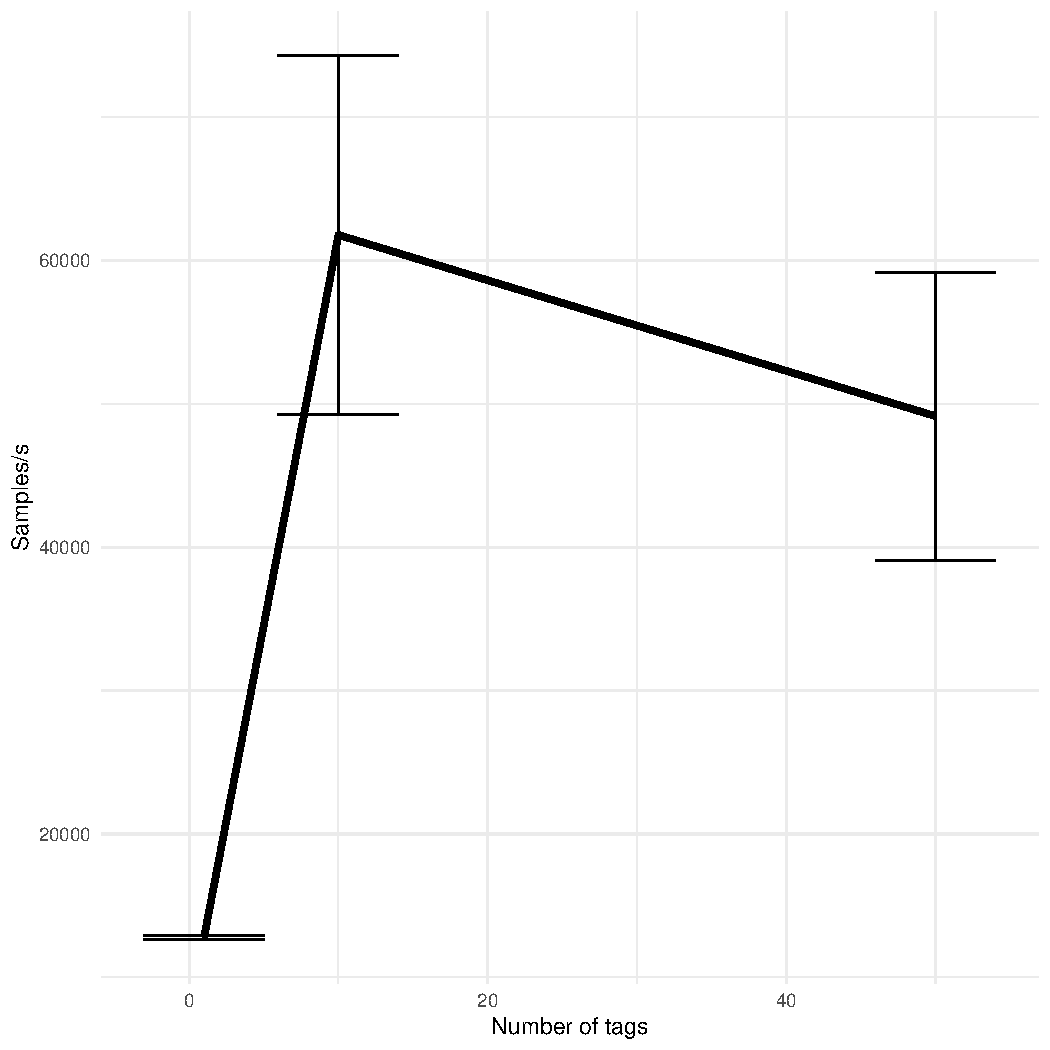
\includegraphics[width=0.45\textwidth]{graphics/write.pdf}
  \caption{Number of datapoints written per second with $95\%$ confidence interval}
  \label{fig:write}
\end{figure}

The same results but for the read performance are shown in Figure~\ref{fig:read}.

\begin{figure}[!hbt]\centering
  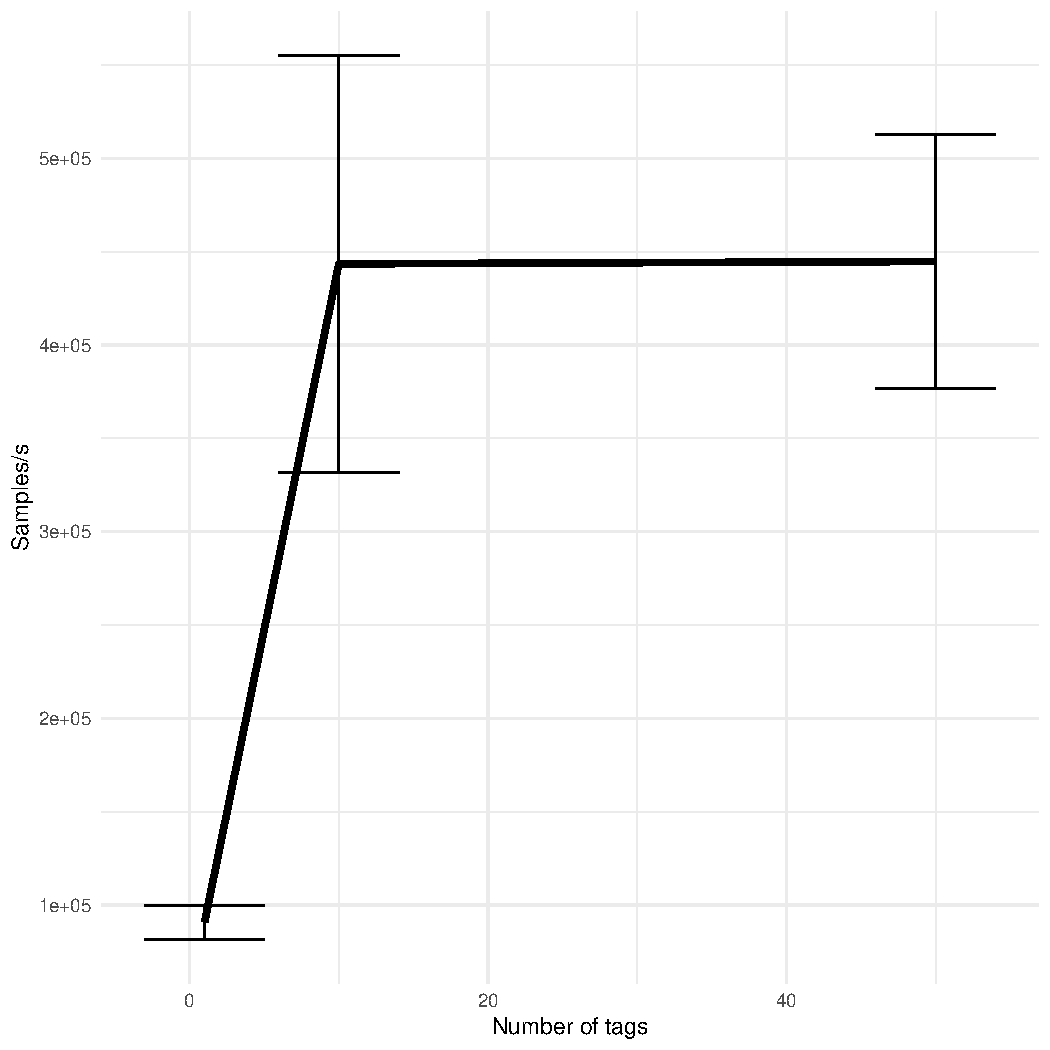
\includegraphics[width=0.45\textwidth]{graphics/read.pdf}
  \caption{Number of datapoints read per second with $95\%$ confidence interval}
  \label{fig:read}
\end{figure}

The results are rather awkward - the read is way much faster than write, which is not
usual for Cassandra database. We will continue to explore this direction further.
